% iaus2esa.tex -- sample pages for Proceedings IAU Symposium document class
% (based on v1.0 cca2esam.tex)
% v1.04 released 17 May 2004 by TechBooks
%% small changes and additions made by KAvdH/IAU 4 June 2004
% Copyright (2004) International Astronomical Union

\NeedsTeXFormat{LaTeX2e}

\documentclass{iau}
\usepackage{graphicx}

\newcommand{\hMpc}{{\ifmmode{h^{-1}{\rm Mpc}}\else{$h^{-1}$Mpc }\fi}}
\newcommand{\hGpc}{{\ifmmode{h^{-1}{\rm Gpc}}\else{$h^{-1}$Gpc }\fi}}
\newcommand{\hmpc}{{\ifmmode{h^{-1}{\rm Mpc}}\else{$h^{-1}$Mpc }\fi}}
\newcommand{\hkpc}{{\ifmmode{h^{-1}{\rm kpc}}\else{$h^{-1}$kpc }\fi}}
\newcommand{\hMsun}{{\ifmmode{h^{-1}{\rm
{M_{\odot}}}}\else{$h^{-1}{\rm{M_{\odot}}}$}\fi}}
\newcommand{\hmsun}{{\ifmmode{h^{-1}{\rm
{M_{\odot}}}}\else{$h^{-1}{\rm{M_{\odot}}}$}\fi}}
\newcommand{\Msun}{{\ifmmode{{\rm {M_{\odot}}}}\else{${\rm{M_{\odot}}}$}\fi}}
\newcommand{\msun}{{\ifmmode{{\rm {M_{\odot}}}}\else{${\rm{M_{\odot}}}$}\fi}}
\newcommand{\lya}{{Lyman$\alpha$~}}
\newcommand{\apj}{ApJ}
\newcommand{\apjs}{ApJS}
\newcommand{\apjl}{ApJL}
\newcommand{\aj}{AJ}
\newcommand{\mnras}{MNRAS}
\newcommand{\mnrassub}{MNRAS accepted}
\newcommand{\aap}{A\&A}
\newcommand{\aaps}{A\&AS}
\newcommand{\araa}{ARA\&A}
\newcommand{\nat}{Nature}
\newcommand{\physrep}{PhR}
\newcommand{\pasp}{PASP}
\newcommand{\pasj}{PASJ} 

\title[The Local Group in the Cosmic Web] %% give here short title %%
{The place of the Local Group in the cosmic web}

\author[Jaime E. Forero-Romero]   %% give here short author list %%
{Jaime E. Forero-Romero$^1$}
\affiliation{$^1$Departamento de F\'isica, Universidad de los Andes, \\ Cra. 1 No. 18A-10, Edificio Ip \\Bogot\'a, Colombia \\ email: {\tt je.forero@uniandes.edu.co} \\[\affilskip]}

\pubyear{2014}
\volume{308}  %% insert here IAU Symposium No.
\pagerange{119--126}
% \date{?? and in revised form ??}
\setcounter{page}{1}
\jname{The Zeldovich Universe: Genesis and Growth of the Cosmic Web}
\editors{R. van de Weygaert, S. Shandarin, E. Saar, J. Einasto, eds.}
\begin{document}

\maketitle

\begin{abstract}
We use the Bolshoi Simulation, a Dark Matter (DM) only cosmological
simulation, to find the most probable place of the
Local Group (LG) in the cosmic web. We use pairs of halos with isolation
and kinematic properties consistent with observations as our LG
simulacra. The cosmic web is defined using a tidal tensor approach. We
find that the LG's prefered location is regions with a DM overdensity
in the range $0<\delta<1$, which makes filaments and sheets the
preferred environment. We find that there is a strong alignment
between the LG and the cosmic web. The orbital angular momentum is
preferetntially perpendicular to the smallest tidal eigenvector. The
vector connecting the two halos is strongly aligned along the
the smallest tidal eigenvector and perpendicular to the
largest tidal eigenvector; the pair lies and moves along
filaments and sheets. We do not find any evidence for an alignment
between the spin of each halo in the pair and the cosmic web. 

\keywords{cosmology: large-scale structure of universe; cosmology:dark matter; cosmology: simulations;  Galaxy: formation}
%% add here a maximum of 10 keywords, to be taken form the file <Keywords.txt>
\end{abstract}

\firstsection % if your document starts with a section,
              % remove some space above using this command.
\section{Introduction}




\section{Finding the cosmic web in numerical simulations}

We use a web finding algorithm based on the tidal tensor computed from
the gravitational potential field computed over a grid. We define the
tensor as:

\begin{equation}
T_{ij} = \frac{\partial^2\phi}{\partial r_{i}\partial r_{j}}, 
\end{equation}
%
where the index $i=1,2,3$ refers to the three spatial directions in
euclidian space and $\phi$ is a normalized gravitational poterntial
that satisfies the following Poisson equation $\nabla^2 \phi=\delta$,
where $\delta$ is the matter overdensity.

The algorithms finds the eigenvalues of this tensor, 
$\lambda_1>\lambda_2>\lambda_3$, and use them to classify each cell in
the grid as a peak, filament, sheet or void if three, two, one or none
of the eigenvectors is larger than a given threshold $\lambda_{\rm
  th}$. Each eigenvalue has associated to it an eigenvector ($e_{1}$,
$e_{2}$, $e_{3}$) which are the natural basis to define local
directions in the web. Details describing the algorithm can be found
in \cite[Forero-Romero et al. (2009)]{Tweb}.




\section{Local Groups in cosmological simulations}
We construct a sample of MW-M31 pairs at $z\sim 0$ by using multiple
snapshots from the simulation asking for consistency with the
following criteria:

\begin{itemize}
\item Relative distance. The distance between the center of mass of
  each halo in the pairs cannot be larger than $1.3$ Mpc.
\item Individual halo mass. Each halo has a mass in the mass range
  $5\times 10^{11}<M_{200c}<5\times 10^{13}\Msun$.  
\item  Isolation. No neighboring halos more massive than either pair
member can be found within $5$Mpc.
\item Isolation from Virgo-like halos. No dark matter halos with mass
  $M_{200c}>1.5\times 10^{14}\Msun$ within $12$Mpc.
\end{itemize}

With the selection criteria we select close to $6\times 10^3$ to build
our main pair sample. From it we select to restricted samples
according to the tolerance in kinematic constraints. These samples 
are named $2\sigma$ and $3\sigma$, and correspond, respectiveley to
two and three times the observational errors in the radial vecloty,
tangential velocity and separation. The number of paris in each sample
is $46$ and $120$. 


\section{The place of the Local Group in the Cosmic Web}

\begin{figure}[b]
% \vspace*{-2.0 cm}
\begin{center}
 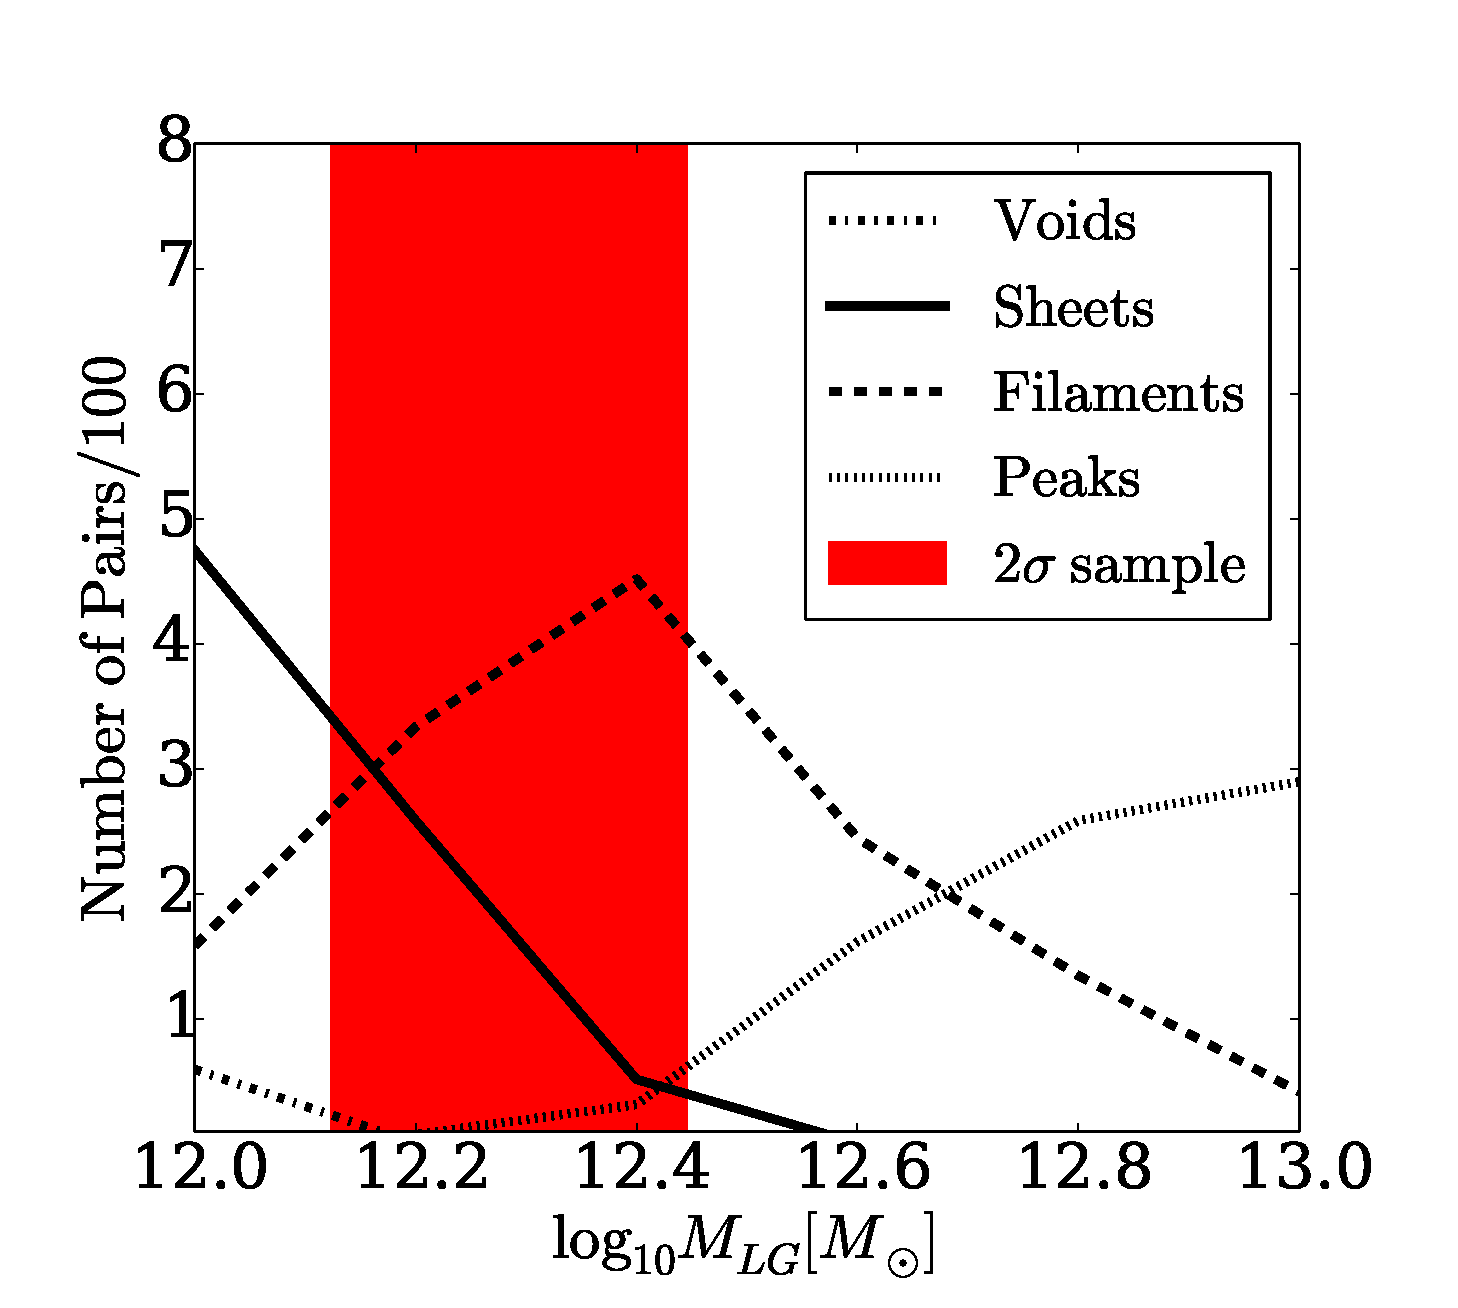
\includegraphics[width=3.8in]{histogram_mass_distro.eps} 
% \vspace*{-1.0 cm}
 \caption{Path of pre-solar grains from their stellar sources to the laboratory.}
   \label{fig1}
\end{center}
\end{figure}

\begin{figure}[b]
% \vspace*{-2.0 cm}
\begin{center}
 \includegraphics[width=3.8in]{median_mass_overdensity.eps} 
% \vspace*{-1.0 cm}
 \caption{Path of pre-solar grains from their stellar sources to the laboratory.}
   \label{fig1}
\end{center}
\end{figure}

\begin{figure}[b]
% \vspace*{-2.0 cm}
\begin{center}
 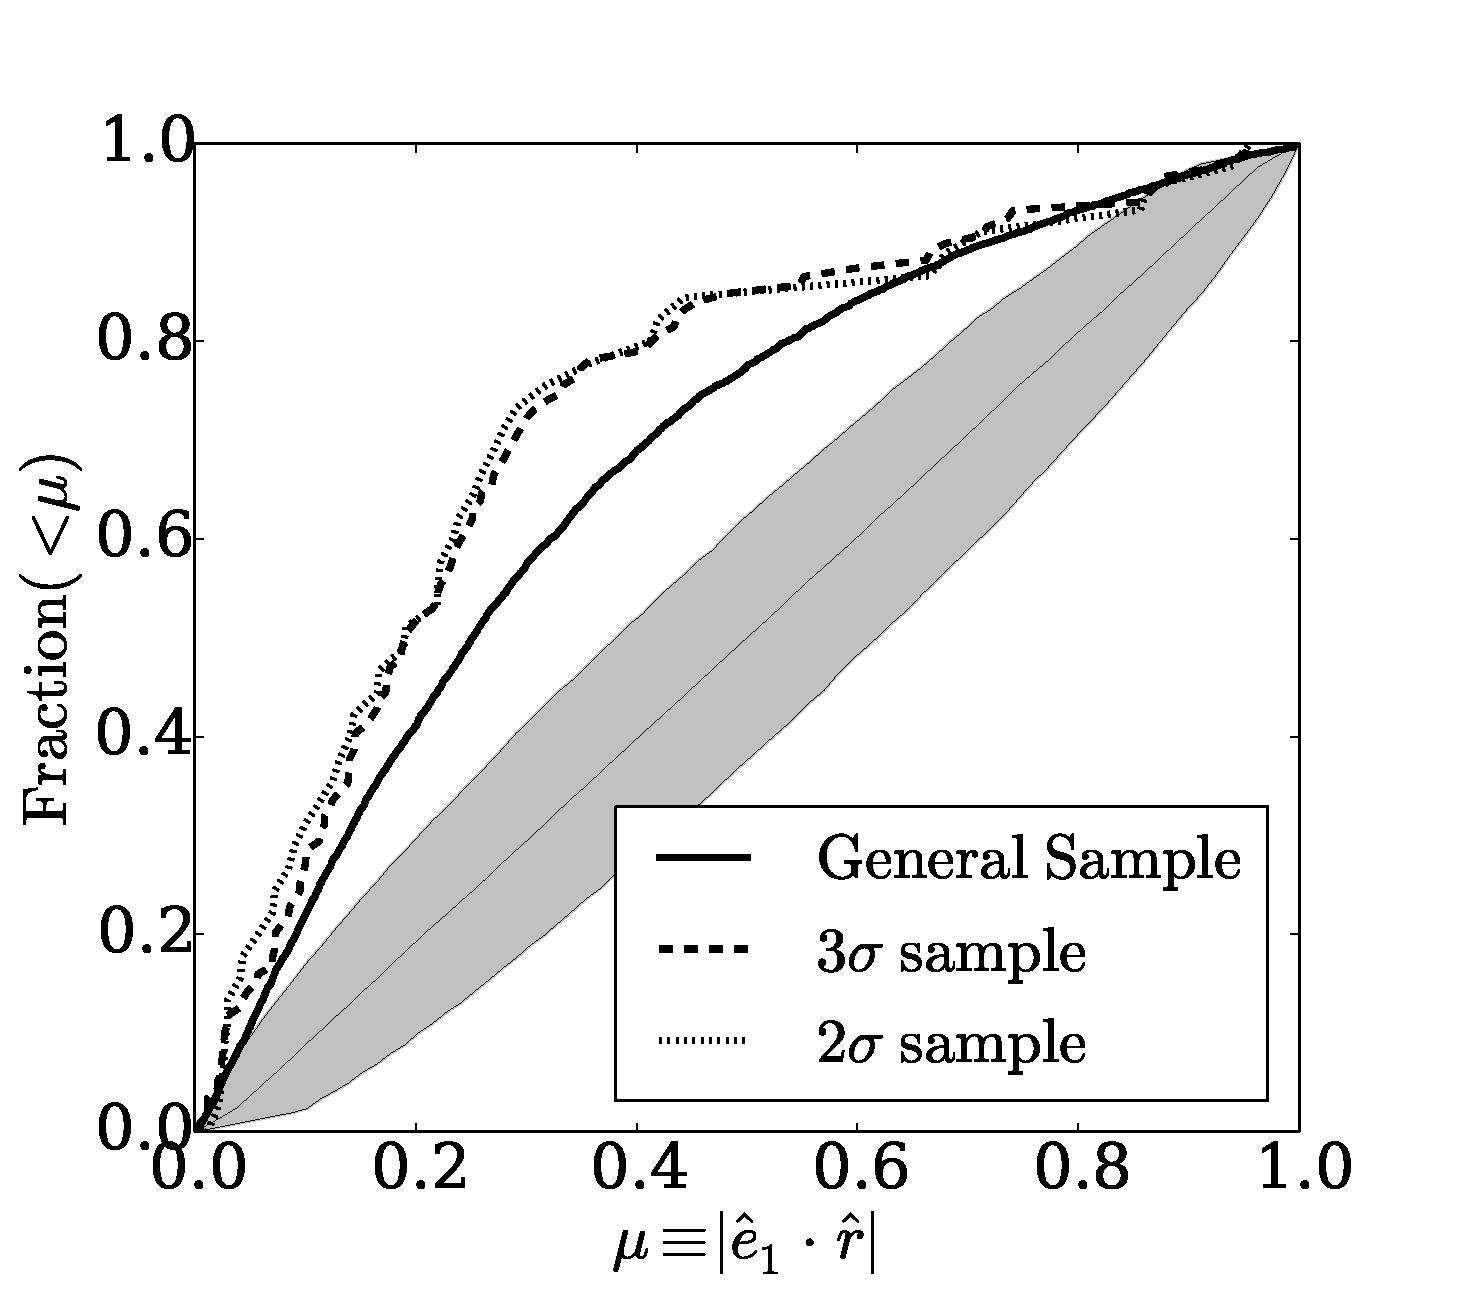
\includegraphics[width=2.6in]{alignments_e1_r_all_environments.eps} 
 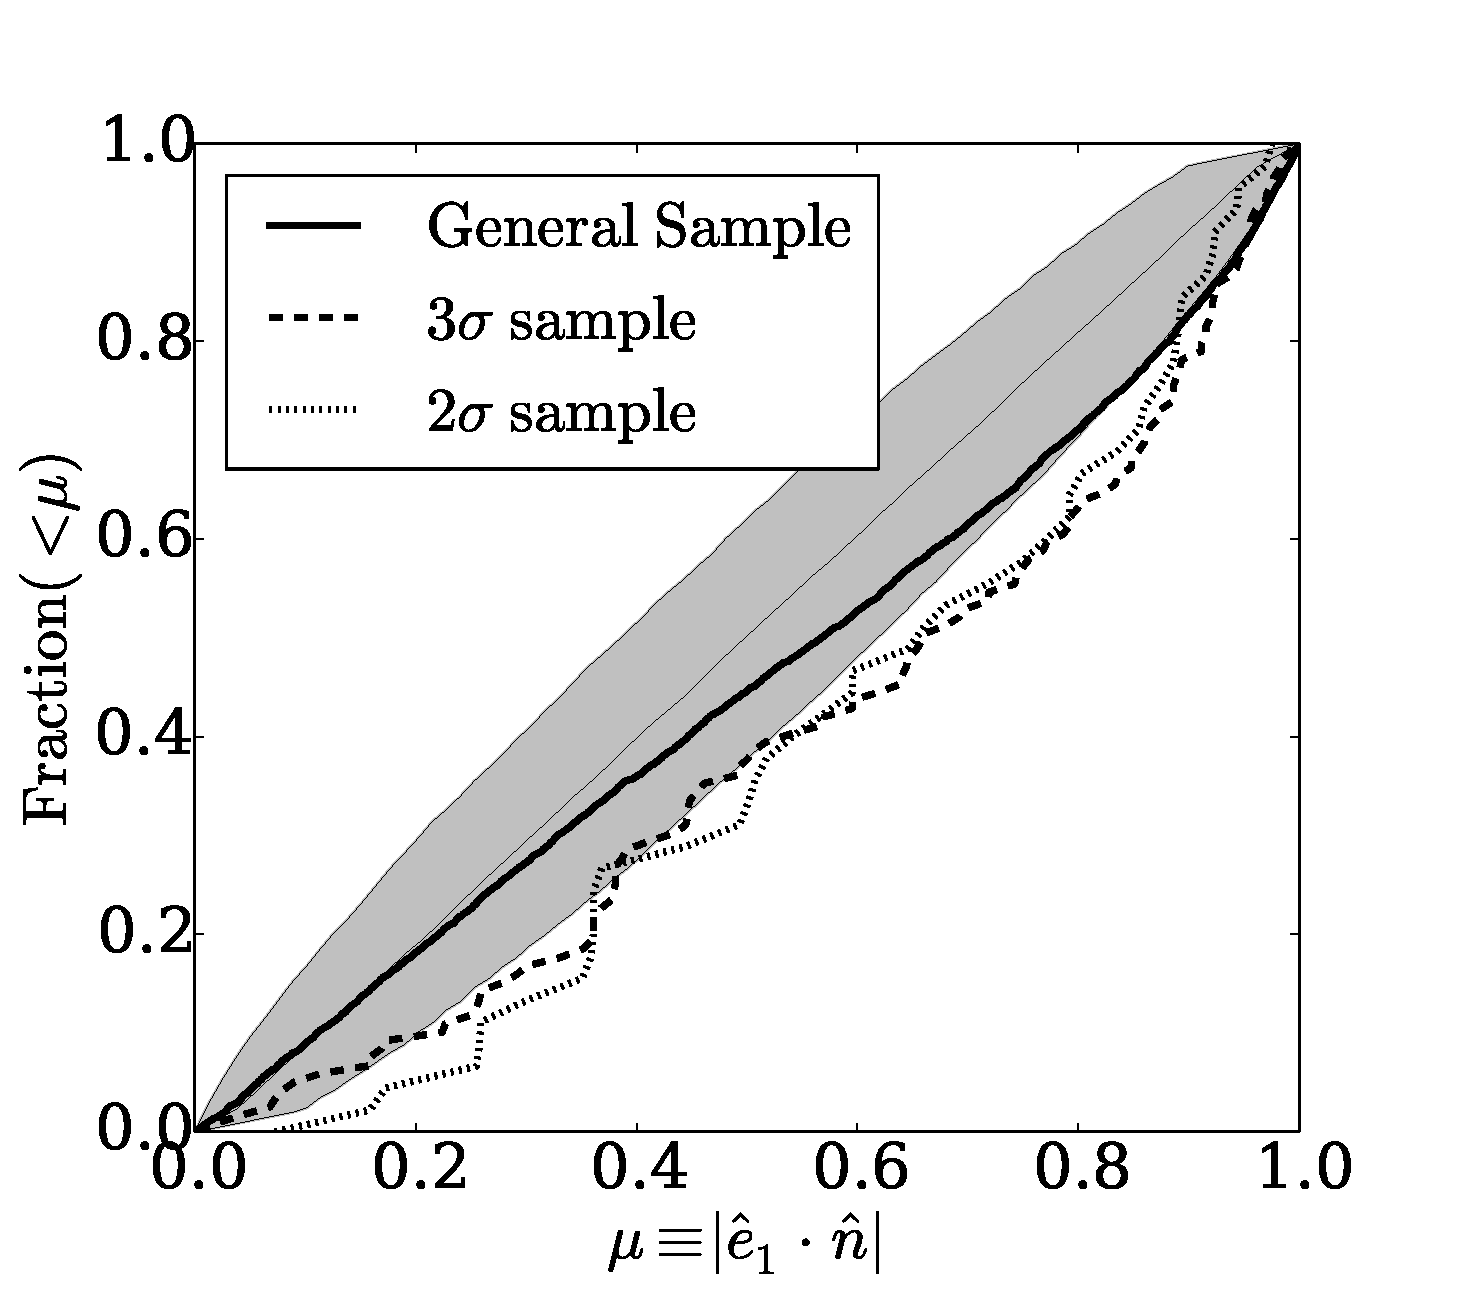
\includegraphics[width=2.6in]{alignments_e1_n_all_environments.eps} 
 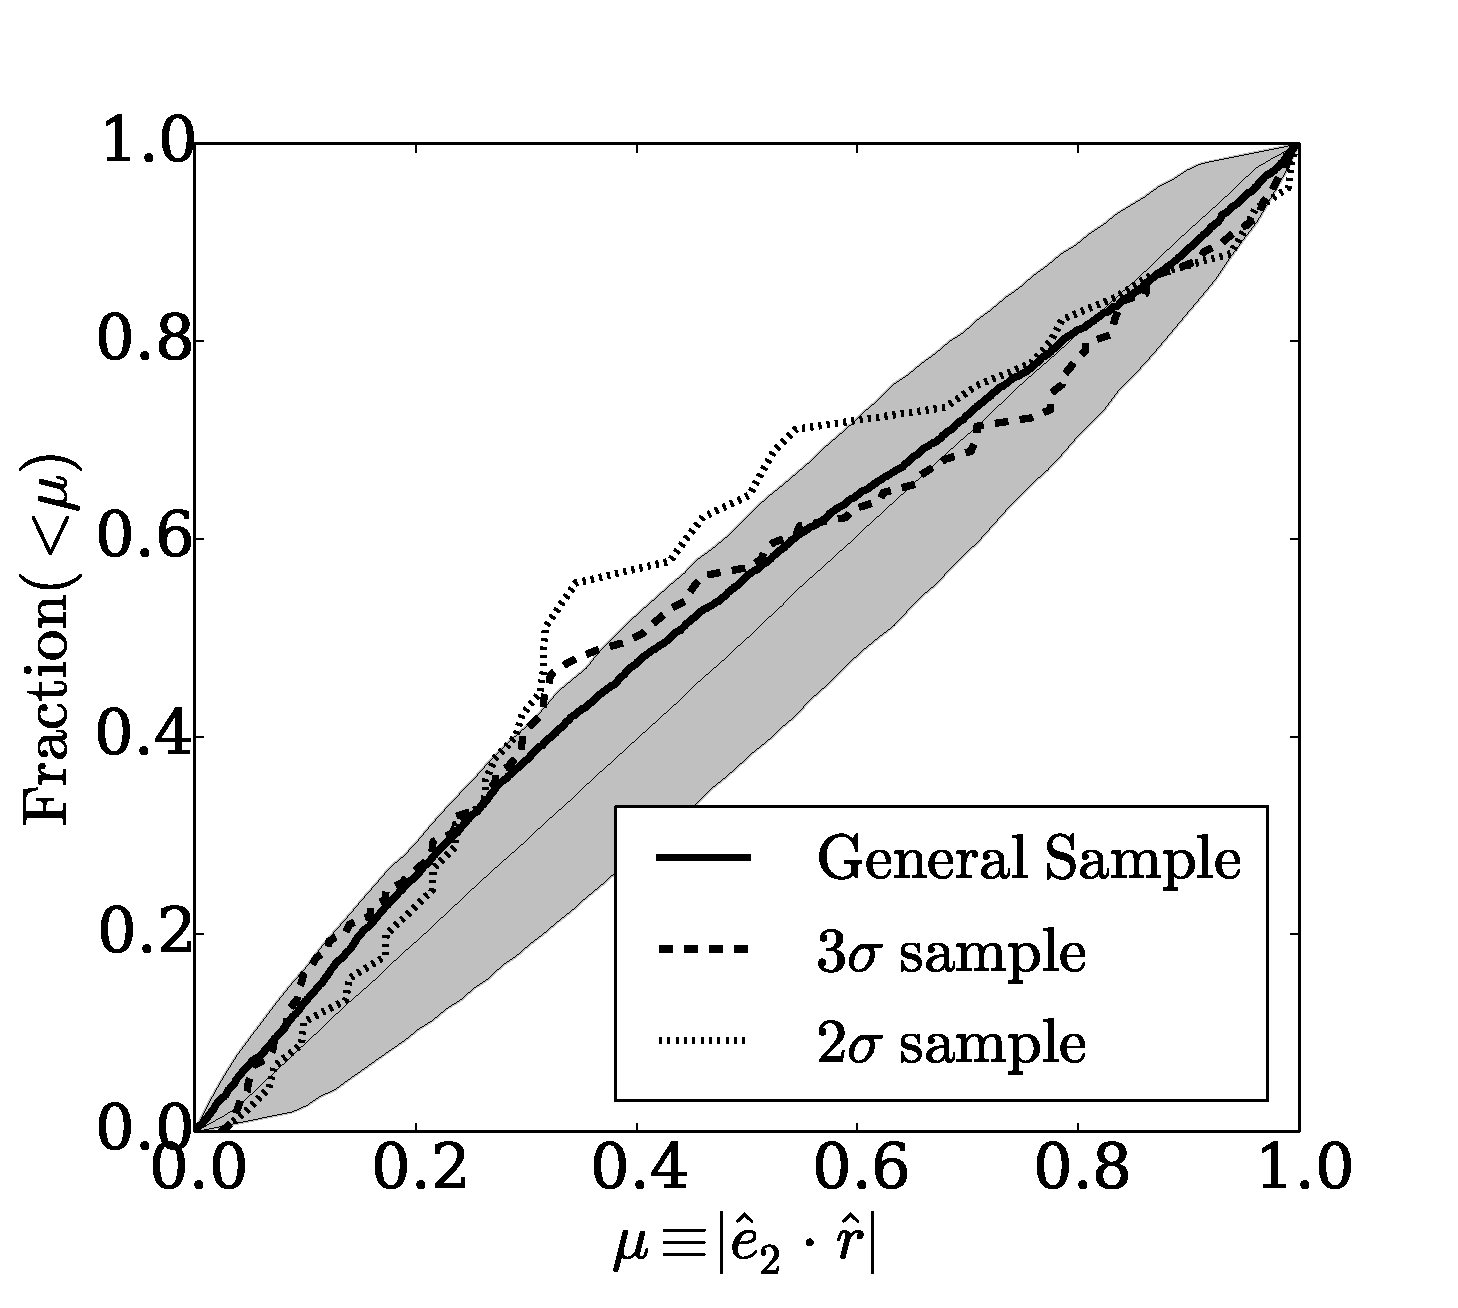
\includegraphics[width=2.6in]{alignments_e2_r_all_environments.eps} 
 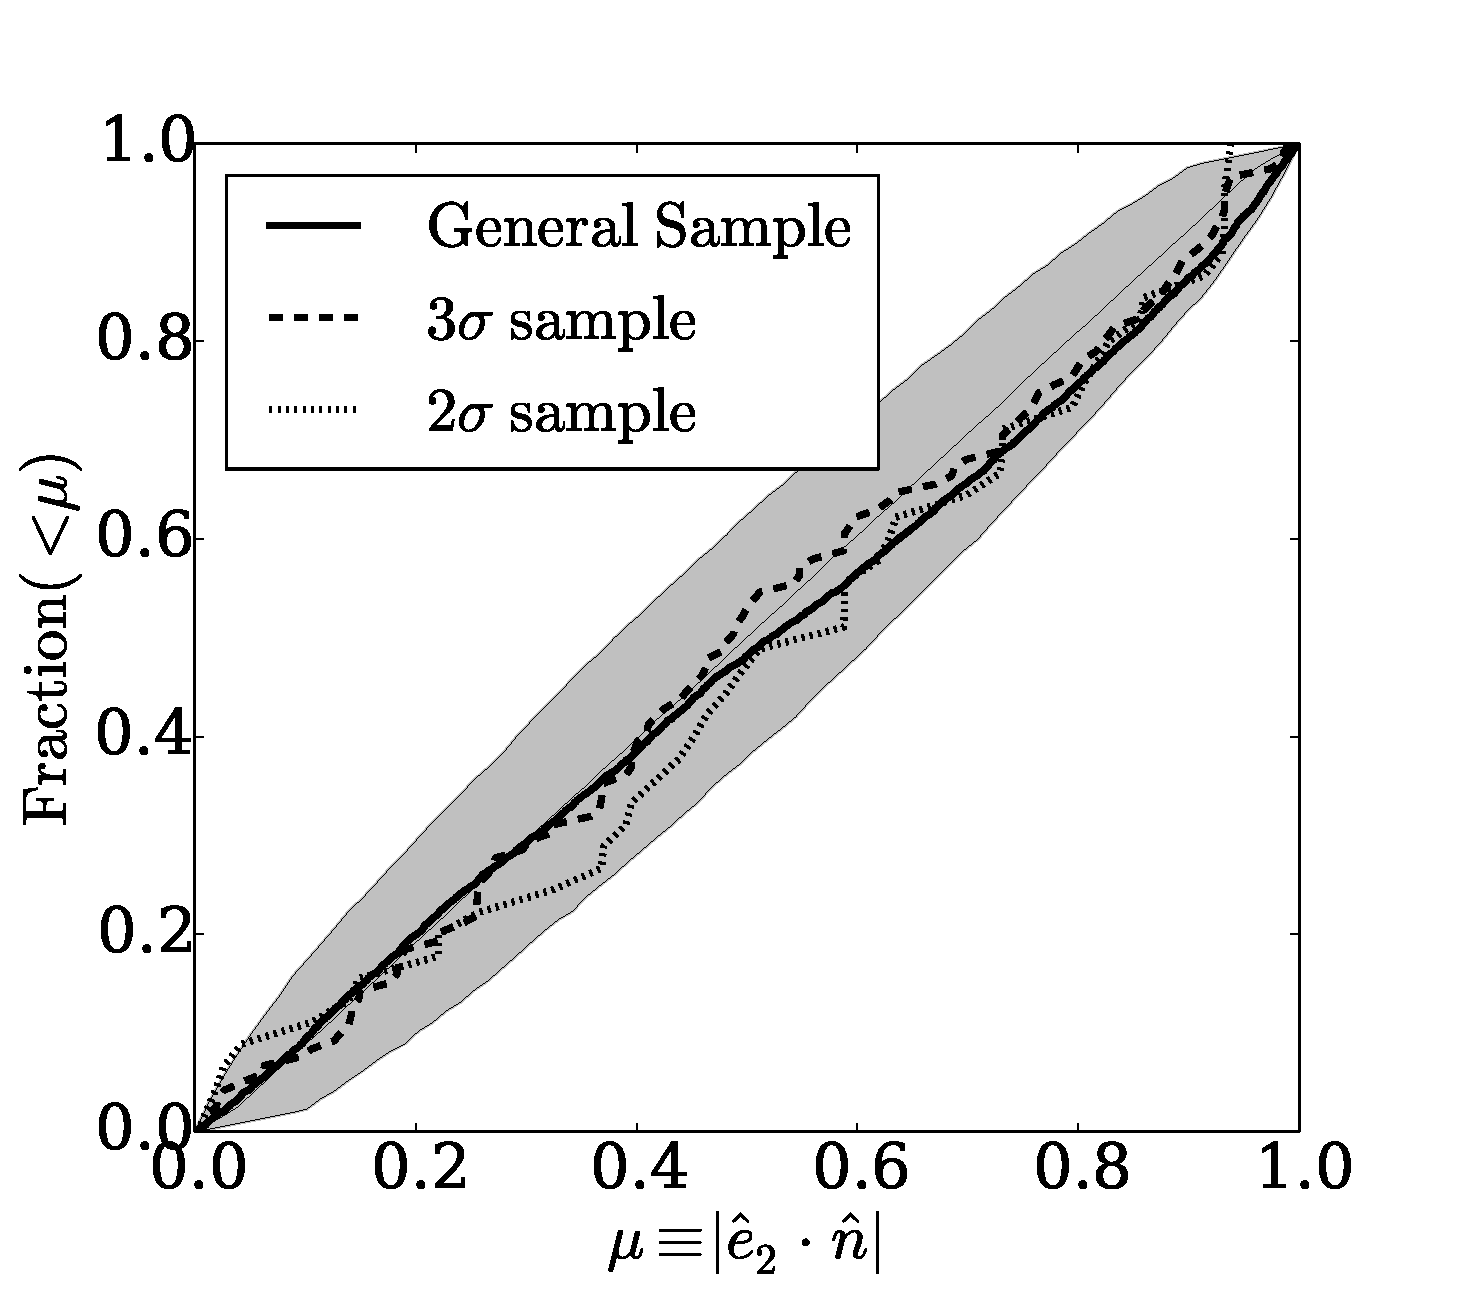
\includegraphics[width=2.6in]{alignments_e2_n_all_environments.eps} 
 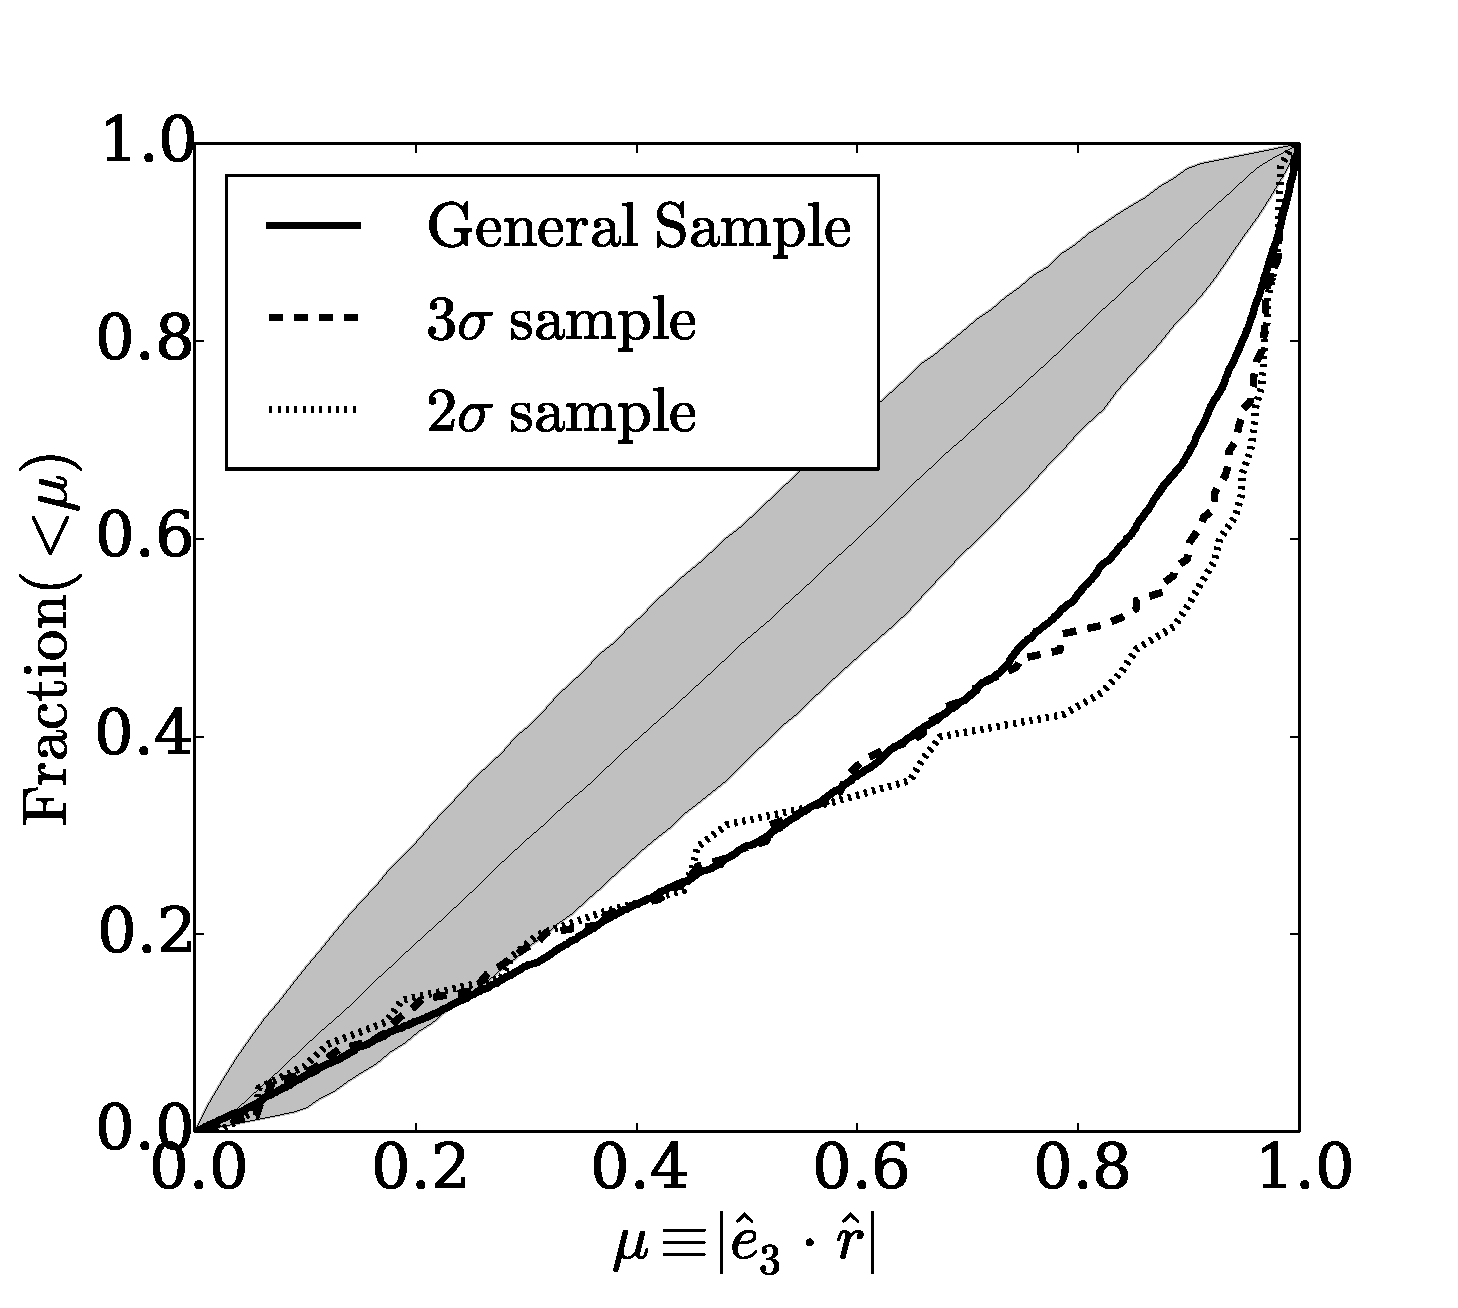
\includegraphics[width=2.6in]{alignments_e3_r_all_environments.eps} 
 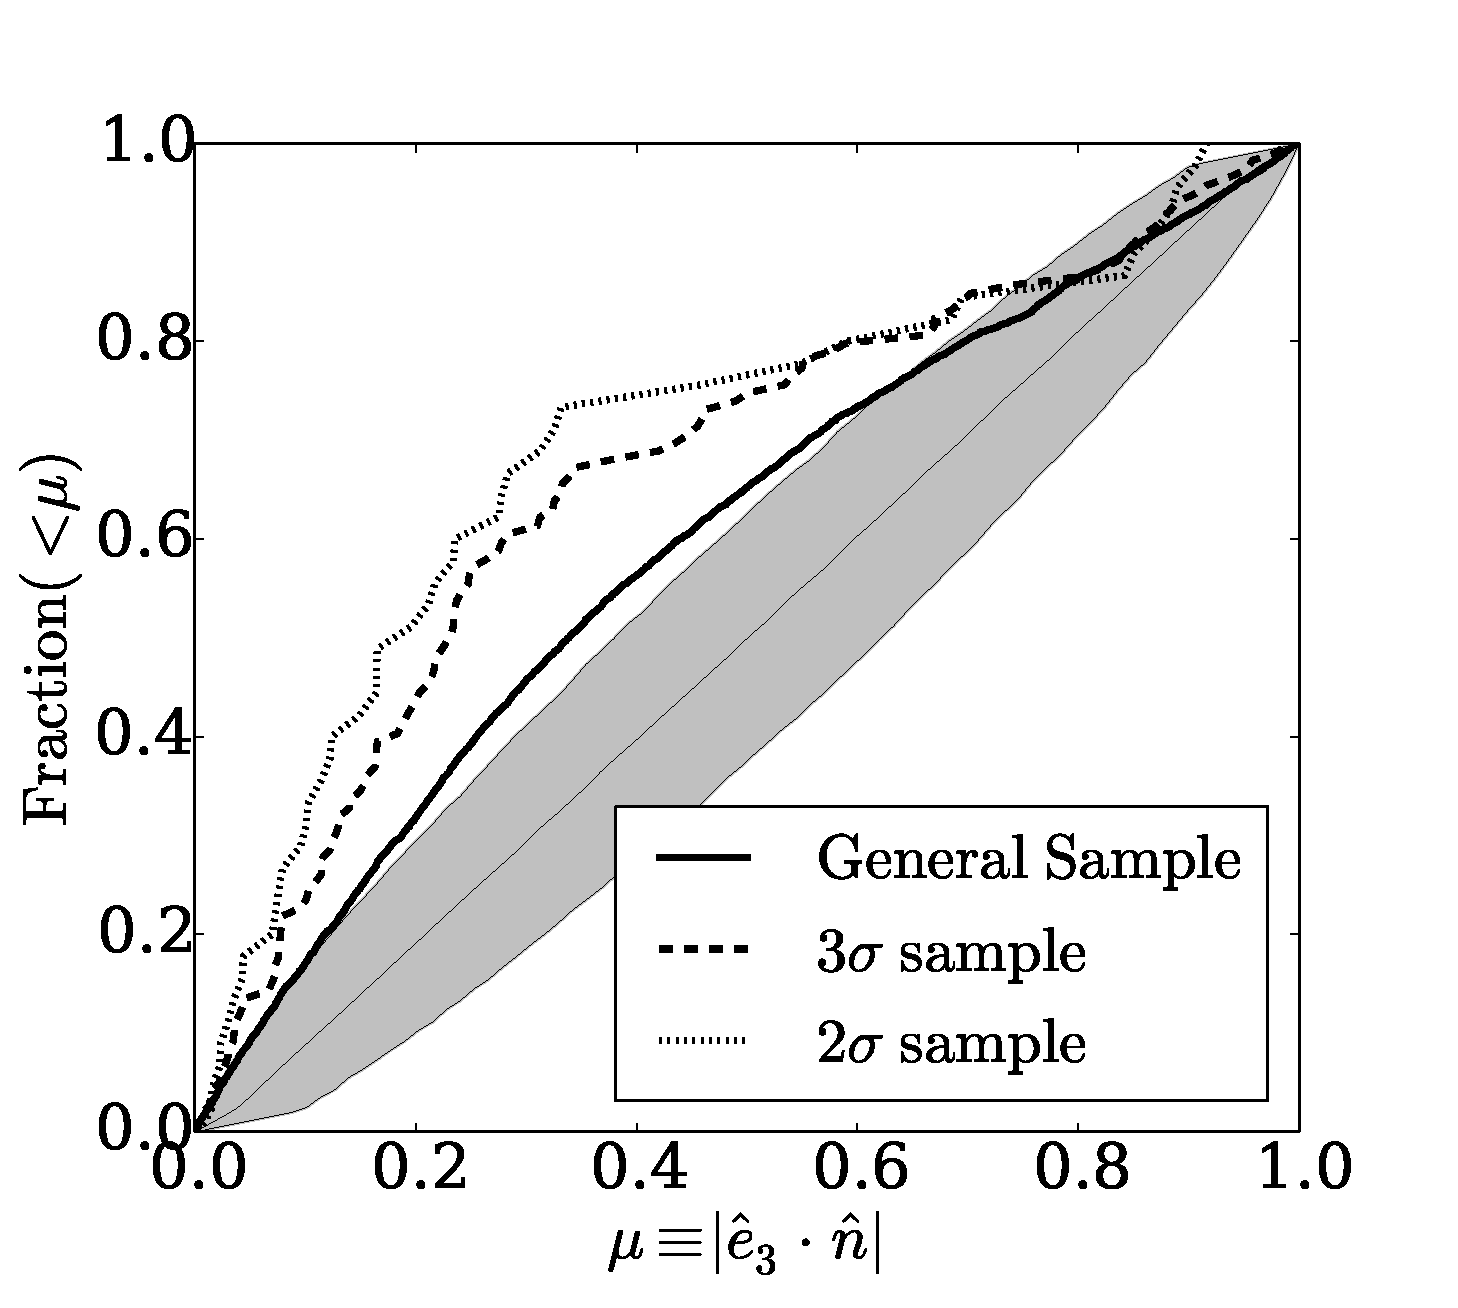
\includegraphics[width=2.6in]{alignments_e3_n_all_environments.eps} 
% \vspace*{-1.0 cm}
 \caption{Path of pre-solar grains from their stellar sources to the laboratory.}
   \label{fig1}
\end{center}
\end{figure}



\section{Alignments with the cosmic web}

There is wide evidence showing that DM halo formation properties only
depend on environment through the local DM density. Whether they are
located in sheet or a filament is irrelevant as long the local density
is the same. 

However there is long story of measuring aligments (shape, spin,
peculiar velocities) of individual halos with the cosmic web. In a
recent paper \cite{ForeroRomero2014} presented a study
using the same simulation we have at hand together with the same
definition for the cosmic web we use here. They also presented a comprehensive
review of all the previous results from simulations that also
inspected the alignment of halo shape and spin. 

The main results from these studies is that shape presents the
strongest alignment signal. In this case the DM halo major axis lies
along the smallest eigenvector $e_{3}$, regardless of the web
environmet. This alignments is stronger for higher halo
masses. Concerning spin alignment the simulations show a weak
antialignment with respect to $e_{3}$ for halo masses larger that
$10^{12}$\Msun, and no alignment signal for masses below that
threshold. The peculiar velocities show a strong alingment signal
along $e_{3}$ for all masses.


In our case we test for the alignment of the orbital angular momentum
of the pair, the vector connecting the two halos and the spin of each
halo. The results are summarized in the Figure XXX


\section{Overview}







\section{Conclusions}

Here, we have summarized results on the expected place of the Local
Group in the cosmic web. Our results are based on cosmological N-body
simulations and the tidal web method to define the cosmic web. We
constructed different Local Groups samples from dark matter halo pairs
that fulfill observational kinematic constraints. 

We found a tight correlation of the LG pairs' total mass with the scalar
web properties (overdensity, ellipticity and prolateness). For the LG
pairs closer to the observational constraints their total mass is in
the range $1\times 10^{12}\Msun < M_{LG} < 4\times 10^{12}\Msun$
preferred overdensity value is constrained to be in the range
$0<\delta <1$. 

We also found a tight aligment of the pairs with the cosmic web. The
vector joining the two LG halos is aligned with the lowest eigenvector
and antialignned with the highest eigenvector. This means that pairs
are aligned along the filaments and lie along sheets. These alignments
are tighter as the pairs' kinematic conditions are closer to
observations.


 

\begin{thebibliography}{}


\bibitem[{{Forero-Romero} {et~al.}(2014){Forero-Romero}, {Contreras}, \&
{Padilla}}]{ForeroRomero2014}
{Forero-Romero}, J.~E., {Contreras}, S., \& {Padilla}, N. 2014, \mnras, 443,
1090

\bibitem[{{Forero-Romero} {et~al.}(2013){Forero-Romero}, {Hoffman},
{Bustamante}, {Gottl{\"o}ber}, \& {Yepes}}]{2013ApJ...767L...5F}
{Forero-Romero}, J.~E., {Hoffman}, Y., {Bustamante}, S., {Gottl{\"o}ber}, S.,
\& {Yepes}, G. 2013, \apjl, 767, L5

\bibitem[{{Forero-Romero} {et~al.}(2009){Forero-Romero}, {Hoffman},
{Gottl{\"o}ber}, {Klypin}, \& {Yepes}}]{Tweb}
{Forero-Romero}, J.~E., {Hoffman}, Y., {Gottl{\"o}ber}, S., {Klypin}, A., \&
{Yepes}, G. 2009, \mnras, 396, 1815

\bibitem[{{Forero-Romero} {et~al.}(2011){Forero-Romero}, {Hoffman}, {Yepes},
{Gottl{\"o}ber}, {Piontek}, {Klypin}, \& {Steinmetz}}]{ForeroRomero2011}
{Forero-Romero}, J.~E., {Hoffman}, Y., {Yepes}, G., {Gottl{\"o}ber}, S.,
{Piontek}, R., {Klypin}, A., \& {Steinmetz}, M. 2011, \mnras, 417, 1434

\bibitem[{{Gonz{\'a}lez} {et~al.}(2013){Gonz{\'a}lez}, {Kravtsov}, \&
{Gnedin}}]{sat}
{Gonz{\'a}lez}, R.~E., {Kravtsov}, A.~V., \& {Gnedin}, N.~Y. 2013, \apj, 770,
96

\bibitem[{{Gonz{\'a}lez} {et~al.}(2014){Gonz{\'a}lez}, {Kravtsov}, \&
{Gnedin}}]{lganalogues}
---. 2014, ApJ in press, http://arxiv.org/abs/1312.2587

\bibitem[{{Gonz{\'a}lez} \& {Padilla}(2010)}]{2010MNRAS.407.1449G}
{Gonz{\'a}lez}, R.~E., \& {Padilla}, N.~D. 2010, \mnras, 407, 1449


\bibitem[{{Hoffman} et~al.}]{Vweb} {Hoffman} Y., {Metuki} O., {Yepes}
  G., {Gottl{\"o}ber} S., {Forero-Romero} J.~E., {Libeskind} N.~I.,
  {Knebe} A., 2012, \mnras, 425, 2049 

\end{thebibliography}


\end{document}
